% Supplementary Note 8 -- paste into si_v0.tex after Supplementary Note 7.
% Figure: figs/fig_snapshot_audit.pdf (built by figs/make_fig_snapshot_audit.py from
% data/snapshot_audit.csv and data/snapshot_audit_50.extxyz; generator
% alchemi_a100_package/scripts/13_snapshot_audit.py, RNG seed 20261007).
\section*{Supplementary Note 8: Stratified random audit of the production trajectories}

To test whether an arbitrary frame of the production runs is a physically sound
Li|LLZO configuration, 50 snapshots were drawn at random from the full
campaign, stratified in time: the 0--5~ns span was cut into ten 0.5~ns
windows and five snapshots were drawn from each. Within a window each draw
took the cell--temperature pair used least so far, then a random replica and
a random frame, so the sample covers the six cells (seed1 10, seed2 9, seed3
10, seed4 7, idx0 7, idx1 7 snapshots) and the four temperatures (500~K 13,
600~K 12, 700~K 13, 800~K 12). Beyond 3.6~ns only seed1--3 exist, because the
job carrying seed4, idx0 and idx1 stopped at 3.59~ns on a GPU fault; five
snapshots from that job were read from its raw trajectory store. The random
seed is fixed, so the same 50 frames are drawn on every run.

Each snapshot was required to pass eight hard checks: (i) boundary conditions
periodic in $x,y$ and open in $z$, with the cell unchanged; (ii) atom counts
equal to the starting structure and no non-finite coordinates or forces;
(iii) no atom pair closer than 0.6 times the sum of covalent radii; (iv) the
largest force on a mobile atom below 10~eV\,\AA$^{-1}$; (v) the instantaneous
kinetic temperature of the mobile atoms within $\pm20\,\%$ of the target;
(vi) no energy spike, defined as a departure from the running median over
$\pm50$~ps larger than five robust standard deviations of that chunk's
residuals; (vii) layer integrity: fewer than 5\,\% of La/Zr/O atoms more than
2~\AA\ above the original oxide top, no atom detached from the slab, fixed
atoms displaced by less than 0.5~\AA, interface plane shifted by less than
3~\AA, and vacuum retained on both open faces; (viii) the LLZO 8--15~\AA\ below
the interface plane still crystalline, with a root-mean-square displacement of
mobile La/Zr/O from the starting structure below 0.75~\AA.

All 50 snapshots pass all eight checks (Supplementary Fig.~\ref{sfig:audit}a);
the closest approach to any limit is 0.87 of the limit, for the shortest La--O
distance. The shortest distances over the sample are Li--Li 1.86, Li--O 1.57,
Zr--O 1.70, La--O 1.89 and O--O 2.48~\AA; the largest force is
6.0~eV\,\AA$^{-1}$ (median 3.5); kinetic temperatures lie within $-11$ to
$+7.5\,\%$ of target; the interior framework displacement is at most
0.45~\AA\ (median 0.28~\AA), against 1.9~\AA\ in the disordered top 3~\AA\ of
the contact. Every side view shows the layer sequence of vacuum, lithium metal,
interface, LLZO and fixed substrate (Supplementary Fig.~\ref{sfig:audit}b).
With no failure in 50 draws, the fraction of unphysical frames in the campaign
is below $1-0.05^{1/50}=5.8\,\%$ at 95\,\% confidence. Frames from the same
trajectory are correlated, so the bound applies to the sampled
cell--temperature--time strata rather than to 50 independent trajectories.

Two expected features are reported but not scored. In seed4 at 800~K,
67--69\,\% of the lithium that started in the metal remains above the interface
plane, because the rest has filled vacancies in the 0.5~vac/f.u.\ oxide (main
text). Energies measured against the first frame of a chunk move by up to
123~meV/atom only in the first chunk, whose first frame is the unheated
starting structure; thereafter the chunk-mean energy of a trajectory is
constant to 1~meV/atom over 5~ns. The 50 frames, with their MACE energies and
forces, are provided as \texttt{snapshot\_audit\_50.extxyz} for independent
first-principles single-point checks.

\begin{figure}[h]
\centering
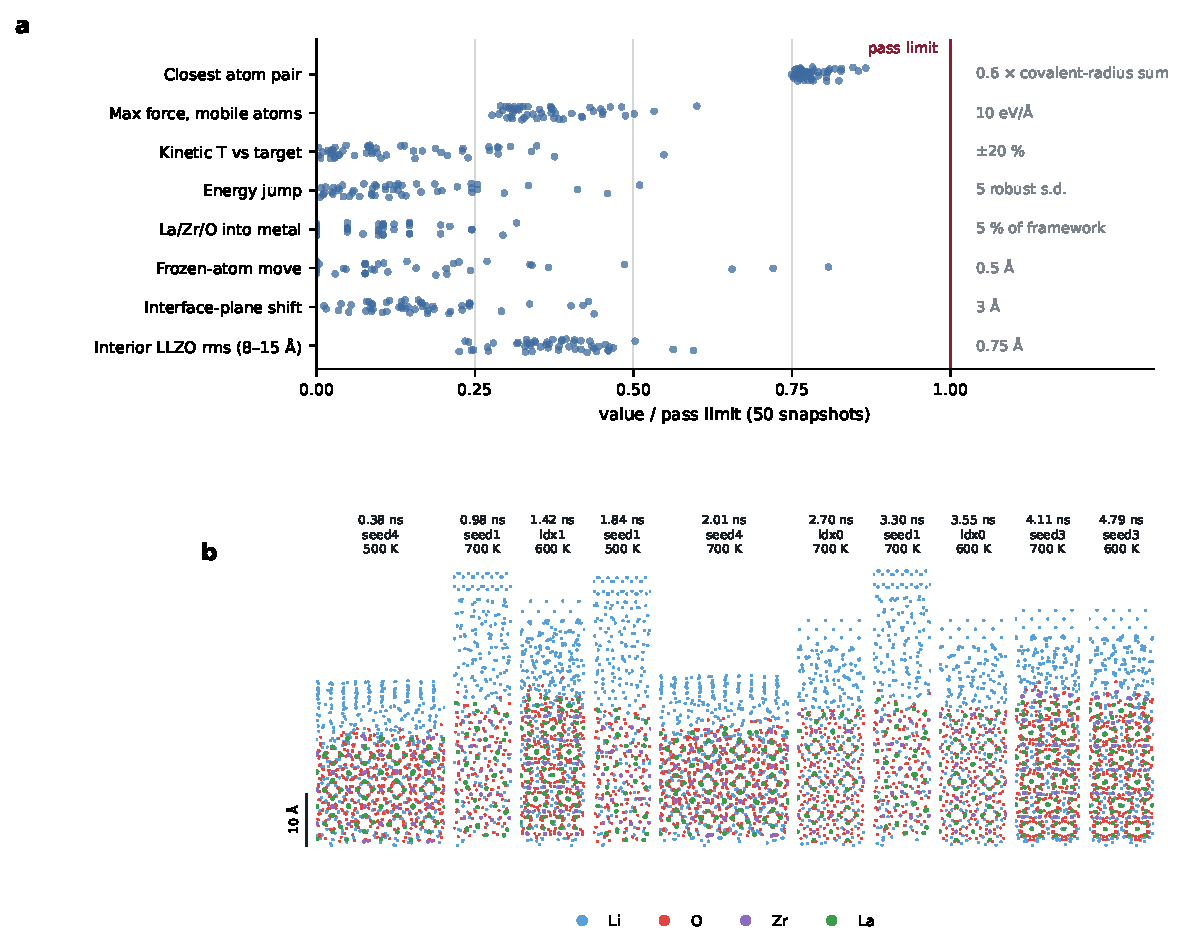
\includegraphics[width=\linewidth]{figs/fig_snapshot_audit.pdf}
\caption{\textbf{Stratified random audit of 50 production snapshots.}
\textbf{a}, Each hard check expressed as a fraction of its pass limit (right),
one dot per snapshot (vertical jitter for visibility); all values lie below 1.
\textbf{b}, Side views ($x$--$z$) of the first snapshot drawn from each 0.5~ns
window, on a common length scale, with simulation time, cell and temperature
above each. Blue Li, red O, green La, purple Zr.}
\label{sfig:audit}
\end{figure}
